\section{Desarrollo}

La Inducción Matemática es una técnica utilizada para probar declaraciones o proposiciones.
La idea es similar a la de hacer caer varias piezas de dominó.
Si cada pieza está lo suficientemente cerca de la anterior y hacemos caer la primera, entonces todas las piezas eventualmente van a caer.
Cuando queremos probar una proposición sobre números naturales, la idea es la misma.
En la Figura~\ref{fig:figure} podemos ver una representación gráfica de esta analogía.

\begin{figure}[htb]
    \centering
    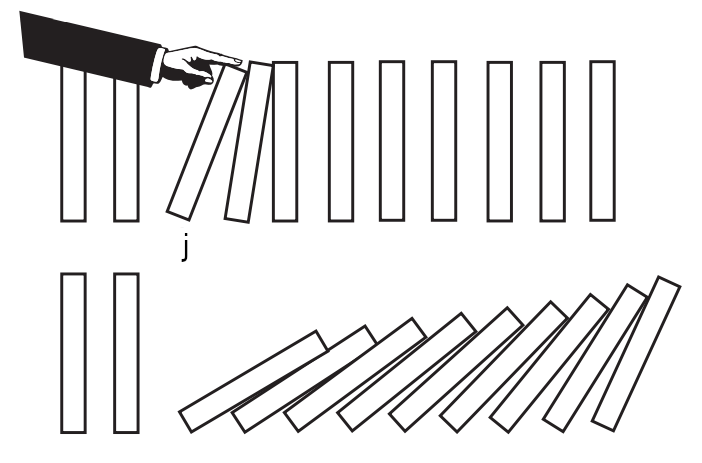
\includegraphics[width=8cm]{images/dominoes-fall}
    \caption{Fichas de dominó cayendo.}
    \label{fig:figure}
\end{figure}

La importancia de la inducción matemática radica que con ella es posible probar proposiciones o propiedades sobre todos los números enteros en función de unos pocos pasos.
Es decir, podemos validar una propiedad a infinitos números en función de unos pasos finitos.

Otra analogía es la siguiente.
Considera una pila de sobres, tan alta como querás.
Supongamos que cada uno de los sobres tiene el mismo mensaje en su interior ``\textit{Abre el siguiente sobre de la pila, y sigue las instrucciones escrito en él}''.
Si alguien abre el primero (el de arriba), lee el mensaje y sigue las instrucciones, entonces la persona se ve obligada a abrir el segundo sobre.
Y si la persona decide seguir cada instrucción, entonces esta persona abrirá todos los sobres de la pila.
Es decir, esto es el principio de Inducción Matemática aplicado a una pila de sobres.

\begin{principle.tcb}{\textbf{Principio de Inducción Matemática}}{}
    Sea algún entero $j$ y sea $S(n)$ una declaración\footnote{También podemos decir Proposición o Afirmación} en función del entero $n$ con $n \geq j$.
    Entonces,
    \begin{itemize}
        \item si $S(j)$ es cierto, y
        \item para cada entero $k \geq j$, $S(k) \implies S(k + 1)$,
    \end{itemize}
    podemos asegurar que la declaración $S(n)$ es cierta para todo $n \geq j$.
\end{principle.tcb}

Una manera de estructurar una prueba por inducción matemática es la siguiente.
\begin{enumerate}
    \item \textbf{[BI] Base de inducción (o caso base)}\\
    Probar que $S(j)$ es cierta (generalmente $j$ será 1, pero dependiendo del problema puede ser -5, 17, 1000 etc.).

    \item \textbf{[HI] Hipótesis de inducción}\\
    Suponer que para un entero $k \geq 1$, la declaración $S(k)$ es cierta (la mayoria de veces el mismo problema nos da la hipótesis).

    \item \textbf{[PI] Paso de inducción}\\
    Probar que como $S(k)$ es cierta esto implica que $S(k + 1)$ también será cierta.
    El paso inductivo muchas veces la parte más compleja de realizar en una prueba por inducción, puesto que muchas veces requiere un conocimiento amplio de matemáticas
\end{enumerate}

\begin{example}
    Sea $m$ entero positivo, probar que para $m \geq 3$, se cumple \[m^m > 2m!.\]
\end{example}

\begin{solution}
    Detonemos la siguiente proposición
    \[
        S(m) : m^m > 2m!,
    \]
    la cual puede cierta o falsa.
    \textbf{[BI]} Tomando $m = 3$ vemos que $S(3) : 3^3 > 2\cdot3!$, por lo tanto para $m = 3$, $S(m)$ es cierta.
    \textbf{[HI]} Ahora, supongamos que para algún entero fijo $k\geq 3$, $S(k)$ es cierta.
    \textbf{[PI]} Como $S(k)$ es cierta entonces probaremos que esto implica a $S(k + 1)$ como cierta.
    Sabemos
    \[
        S(k + 1) : (k + 1)^{k + 1} > 2(k + 1)!,
    \]
    descomponiendo esta expresión vemos que
    \begin{align*}
    (k + 1)
        ^{k}\cdot(k + 1)^1 &> 2(k + 1)\cdot k!\\
        (k + 1)^k &> 2k!
    \end{align*}
    Ahora bien, como $k$ es entero claramente $k + 1 > k$, por lo tanto $(k + 1)^k > k^k$.
    Así por la hipótesis de inducción lo siguiente se cumple
    \[
        (k + 1)^k > k^k > 2k!.
    \]
    Hemos probado que si $S(k)$ es cierta esto implica que $S(k + 1)$ también es cierto, por tanto $S(m)$ es cierto para todo $m \leq 3$.
    Luego, la prueba está hecha.
\end{solution}

\begin{theorem.tcb}{\textbf{Binomio de Newton}}{}
    Sea $a$ y $b$ números reales y $n$ un entero no negativo, se cumple que
    \[
        (a + b)^n = \binom{n}{0}a^n + \binom{n}{1}a^{n - 1}b + \cdots + \binom{n}{i}a^{n - i}b^i + \cdots + \binom{n}{n}b^n =
        \sum\limits_{i = 0}^{n} \binom{n}{i}a^{n - i}b^i.
    \]
\end{theorem.tcb}

\begin{proof}
    Procederemos por inducción sobre $n$.
    Para $n = 0$ se cumple, ya que $(a + b)^0 = 1$ y $\binom{0}{0}a^0 b^0 = 1$.
    Supongamos que para un entero $k \geq 0$ también se cumple, esto es
    \[
        (a + b)^k = \sum\limits_{i = 0}^{k} \binom{k}{i}a^{k - i}b^i.
    \]
    Probaremos entonces que para $(k + 1)$ también se cumple
    \begin{align*}
    (a + b)
        ^{k + 1} &= (a + b)(a + b)^k = (a + b) \sum\limits_{i = 0}^{k} \binom{k}{i}a^{k - i}b^i\\
        &= a\sum\limits_{i = 0}^{k} \binom{k}{i}a^{k - i}b^i + b\sum\limits_{i = 0}^{k} \binom{k}{i}a^{k - i}b^i\\[2mm]
        &= a\left[\binom{k}{0}a^{k} + \sum\limits_{i = 1}^{k} \binom{k}{i}a^{k - i}b^i\right] + b\left[\sum\limits_{i = 0}^{k - 1} \binom{k}{i}a^{k - i}b^i + \binom{k}{k}b^k\right]\\[2mm]
        &= \binom{k}{0}a^{k + 1} + \left[\sum\limits_{i = 1}^{k} \binom{k}{i}a^{k + 1 - i}b^i+ \sum\limits_{i = 0}^{k - 1} \binom{k}{i}a^{k - i}b^{i + 1}\right] + \binom{k}{k}b^{k + 1} \\[2mm]
        &= \binom{k}{0}a^{k + 1} + \left[\sum\limits_{i = 1}^{k} \binom{k}{i}a^{k + 1 - i}b^i+ \sum\limits_{i = 1}^{k} \binom{k}{i - 1}a^{k + 1 - i}b^{i}\right] + \binom{k}{k}b^{k + 1} \\[2mm]
        &= \binom{k + 1}{0}a^{k + 1} + \sum\limits_{i = 1}^{k} \left[ \binom{k}{i} + \binom{k}{i - 1}\right] a^{k + 1 - i}b^i + \binom{k + 1}{k + 1}b^{k + 1} \\[2mm]
        &= \binom{k + 1}{0}a^{k + 1} + \sum\limits_{i = 1}^{k} \binom{k + 1}{i} a^{k + 1 - i}b^i + \binom{k + 1}{k + 1}b^{k + 1} \\[2mm]
        &= \boxed{\sum\limits_{i = 0}^{k + 1} \binom{k + 1}{i} a^{k + 1 - i}b^i}
    \end{align*}
    Por lo tanto, podemos concluir que $(a + b)^n = \sum\limits_{i = 0}^{n} \binom{n}{i}a^{n - i}b^i$ se cumple para todo $n \in \Z^{\geq 0}$.
\end{proof}

La \textbf{Inducción fuerte} es el principio general de la inducción matemática.
Esta surge cuando para probar $S(k + 1)$ no es suficiente considerar $S(k)$ si no que resulta necesario considerar más de una proposición anterior como cierta $S(i), S(i + 1), \cdots, S(k)$.
Muchas veces no hace falta usar todas las declaraciones anteriores, pero sí al menos un par de ellas (dependerá del problema).


\section{Ejercicios y Problemas}

Sección de ejercicios y problemas para el autoestudio.

\showLine
\begin{multicols}{2}

    \begin{exercise}{(Un clásico)}
        Probar que
        \[
            1 + 2 + \dots + n = \dfrac{n(n+1)}{2}
        \]
        para todo $n \in \Z^{\geq 0}$.
    \end{exercise}

    \begin{exercise}
        Probar que se cumple
        \[
            1^2 + 2^2 + \dots + n^2 = \dfrac{n(n+1)(2n+1)}{6}
        \]
        para todo $n \in \Z^{\geq 0}$.
    \end{exercise}

    \begin{exercise}
        Calcular
        \[
            S_n = 1 \cdot 1! + 2 \cdot 2! + 3 \cdot 3! + \ldots + n \cdot n!.
        \]
    \end{exercise}

    \begin{exercise}
        Sea
        \[
            S_n = 1 - 2^2 + 3^2 - 4^2 + \ldots + (-1)^{n - 1} n^2,
        \]
        con $n \in \N$, probar $S_k = (-1)^{n - 1} \dfrac{n(n+1)}{2}$.
    \end{exercise}

    \begin{exercise}
        Determinar $u_n$ si $u_1 = 1$ y que $u_n = u_{n + 1} + 3$.
    \end{exercise}

    \begin{exercise}
        Demostrar que si $v_0 = 2$, $v_1 = 3$ y $v_{k + 1} = 3v_k - 2 v_{k - 1}$ para todo número natural $k$, se tiene $v_n = 2^n + 1$.
    \end{exercise}

    \begin{exercise}
        Se habla lo siguiente
        \begin{itemize}
            \item \textbf{Brisa Marina:} Y vos Gerald, te me hiciste el loco con los reales que me debés.
            \item \textbf{Gerald:} Qué fregás, si te los voy a pagar.
            \item \textbf{Brisa Marina:} Pero ideay, cuándo.
            \item \textbf{Gerald:} Dale pues, ya te los doy.
        \end{itemize}
        Si a Brisa Marina le debén más 7 pesos y Gerald solo tiene monedas falsas de 3 y 5 pesos, probar que siempre hay alguna manera de que Gerald ``pague'' la deuda.
    \end{exercise}

    \begin{exercise}
        Sea $\{a_n\}$ con $n \in \N$ una secuencia tal que
        \begin{align*}
            a_1 &= 5\\
            a_2 &= 13\\
            a_{n + 2} &= 5a_{n + 1} - 6a_n
        \end{align*}
        Probar que $a_n = 2^n + 3^n$ para todo $n \in \N$.
    \end{exercise}

    \begin{exercise}
        Probar que $4007^n - 1$ es divisible por 2003 para todo $n \in \Z^{\geq 0}$
    \end{exercise}

    \begin{exercise}
        Demostrar $\forall n \in \N$, que
        \begin{gather*}
            9 \mid 2^{2n} + 15n - 1 \quad
            8 \mid 3^{2n + 2} + 8n - 9
        \end{gather*}
    \end{exercise}

    \begin{exercise}
        Probar para todo $n \in \N$ que el número $A_n = 3^n - 2n^2 - 1$ es múltiplo de $8$.
        Además, si $3\nmid n$, entonces $A_n$ es múltiplo de 24.
    \end{exercise}

    \begin{exercise}
        Sea $(q \neq 1) \in \R$ y sea $n$ un entero no negativo, probar que
        \[
            (1 + q)(1 + q^2)(1 + q^4)\cdots(1 + q^{2^n}) = \frac{1 - q^{2^{n + 1}} }{1 - q}.
        \]
    \end{exercise}

    \begin{exercise}
        Probar para todo $n\geq 2$ natural se cumple $\left(1 - \frac{1}{4}\right) \left(1 - \frac{1}{9}\right) \cdots \left(1 - \frac{1}{n^2}\right) = \frac{n + 1}{2n}.$
    \end{exercise}

    \begin{exercise}
        Demostrar que
        \[
            \frac{1}{n + 1} + \frac{1}{n + 2} + \cdots + \frac{1}{2n} > \frac{13}{24}
        \]
        para todo número natural $n > 1$.
    \end{exercise}
    \begin{exercise}
        Demostrar que $\forall a, b\in \R^+$ se cumple $2^{n - 1}(a^n + b^n) \geq (a + b)^n$ con $n$ natural.
    \end{exercise}

    \begin{exercise}
        Sea $\alpha + \beta = m$ y $\alpha \beta = a$ se define como $A_1 = m - 1$ y
        \[
            A_{k + 1} = m - \dfrac{a}{A_k} \quad (m \neq 1;\ \alpha \neq \beta)
        \]
        con $k > 1$, demostrar que
        \[
            A_n = \frac{(\alpha^{n + 1} - \beta^{n + 1}) - (\alpha^n - \beta^n)}{(\alpha^n - \beta^n) - (\alpha^{n - 1} - \beta^{n - 1})}.
        \]
    \end{exercise}
\end{multicols}